\documentclass[journal]{IEEEtran}
\usepackage{color}
\usepackage[T1]{fontenc}
\usepackage{amssymb,amsmath,amsfonts}
\usepackage{pgfplots}
\usepgfplotslibrary{colormaps}
\pgfplotsset{
    compat=newest,
	colormap={justblackandwhite}{color=(white) color=(white) color=(white)}
}

\begin{document}

    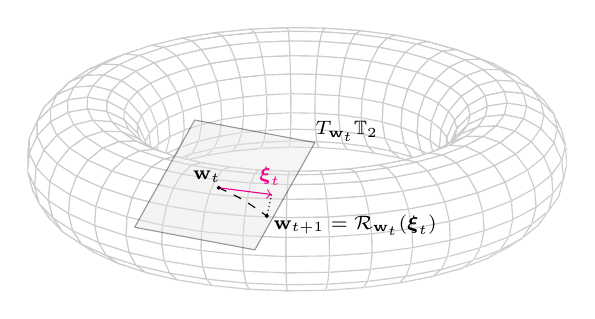
\begin{tikzpicture}

    \begin{axis}[
        axis equal image,
        hide axis,
        z buffer = sort,
        view = {0}{20},
        scale = 1
        ]

        \addplot3[
            surf,
            shader    = faceted interp,
            samples   = 20,
            samples y = 40,
            domain    = 0:2*pi,
            domain y  = 0:2*pi,
            colormap name = justblackandwhite, thin
        ] (
            {(3.5+sin(deg(\x)))*cos(deg(\y))},
            {(3.5+sin(deg(\x)))*sin(deg(\y))},
            {cos(deg(\x))}
        );



    	\addplot3[mark=*,mark size=0.5pt, only marks,draw=black,fill=black] coordinates {
        % (0,  0   , 0) % centre du tore
        %(3.30,  0   , 0) % gauche droite
        %(0,  3   , 0) % profondeur -> doit être à 0 tout le temps
        %(0,  0   , 3) % hauteur 
        (-1.3, 0, -0.5) % point 1 with tangent
        (-0.5,    0, -1) % point2
	    };

        \draw [fill=gray!20,opacity=0.4] 
        (-2.7,0,-1.2) -- (-0.7,0,-1.6) -- (0.3,0,0.3) -- (-1.7,0,0.7) -- (-2.7,0,-1.2);


        \draw [dashed]
        (-1.3, 0, -0.5) .. controls (-0.9,0,-0.7) ..  (-0.5,    0, -1);

       \draw [->, color = magenta] (-1.3, 0, -0.5) -- (-0.42, 0, -0.62);

       \draw [densely dotted] (-0.42, 0, -0.62) -- (-0.5,    0, -1);


    \node[font=\scriptsize, anchor=south west] at (0.15,0,0.15) {${T}_{\mathbf{w}_t} \mathbb{T}_2$};
    \node[font=\scriptsize] at (-1.5, 0, -0.3) {$\mathbf{w}_t$};
    \node[font=\scriptsize] at (-0.45, 0, -0.3) {\textcolor{magenta}{$\boldsymbol{\xi}_t$}};
    \node[font=\scriptsize, anchor=north west] at (-0.55, 0,-0.8) {$\mathbf{w}_{t+1}=\mathcal{R}_{\mathbf{w}_t}(\boldsymbol{\xi}_t) $};

    \end{axis}

    \end{tikzpicture}

\end{document}